\documentclass[tikz,border=10pt]{standalone}
\usetikzlibrary{arrows.meta, positioning, calc}
\usepackage{amssymb}

\begin{document}
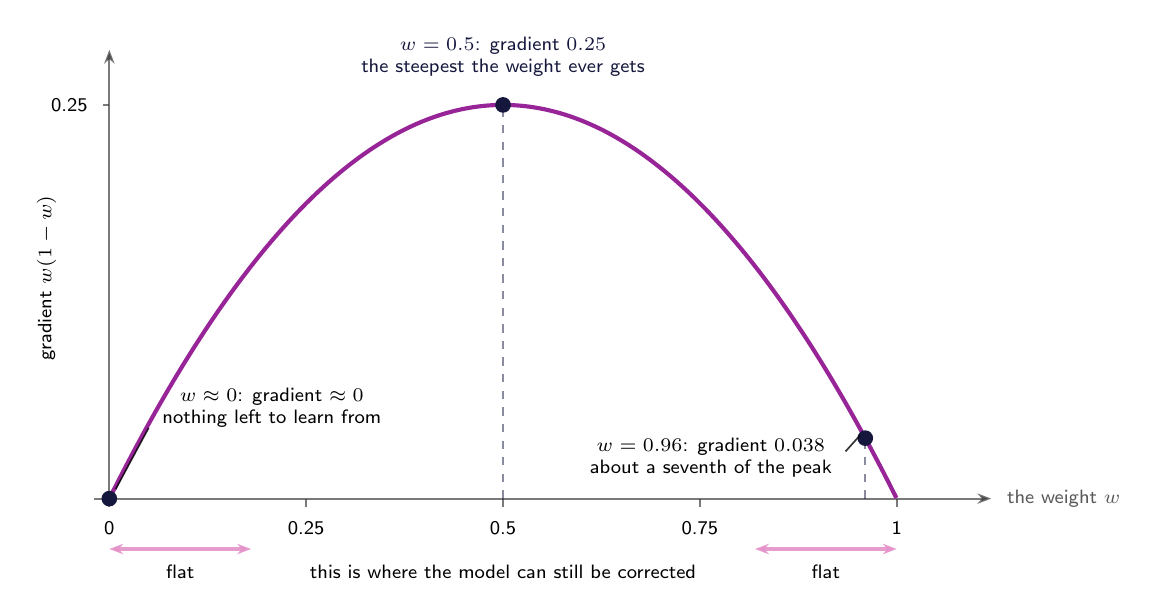
\begin{tikzpicture}[
    every node/.style={font=\sffamily},
    % data coordinates: w in [0,1] -> 10cm wide, w(1-w) in [0,0.25] -> 5cm tall
    x=10cm, y=20cm,
]

% ---------------------------------------------------------------- colours
\definecolor{c1}{HTML}{15173D}
\definecolor{c2}{HTML}{982598}
\definecolor{c3}{HTML}{E491C9}
\definecolor{c4}{HTML}{F1E9E9}
\definecolor{axiscolor}{HTML}{333333}
\definecolor{labelcolor}{HTML}{000000}
\definecolor{deadred}{HTML}{000000}

\tikzset{
    axis/.style={-{Stealth[length=5pt]}, line width=0.8pt, axiscolor,
                 opacity=0.65},
    curve/.style={c2, line width=1.5pt},
    dot/.style={circle, fill=c1, inner sep=2pt},
    drop/.style={c1, line width=0.6pt, dashed, opacity=0.5},
}

% ---------------------------------------------------------------- axes
\draw[axis] (-0.02, 0) -- (1.12, 0)
    node[anchor=west, font=\sffamily\scriptsize, text=labelcolor,
         xshift=2pt] {the weight $w$};
\draw[axis] (0, -0.004) -- (0, 0.285);
\node[font=\sffamily\scriptsize, text=labelcolor, rotate=90, anchor=south]
    at (-0.055, 0.14) {gradient $w(1-w)$};

% ticks on w
\foreach \w/\lab in {0/0, 0.25/0.25, 0.5/0.5, 0.75/0.75, 1/1} {
    \draw[axiscolor, opacity=0.65, line width=0.7pt] (\w, 0) -- (\w, -0.005);
    \node[font=\sffamily\scriptsize, text=labelcolor, anchor=north,
          yshift=-2pt] at (\w, -0.005) {\lab};
}
% ticks on the gradient
\foreach \g/\lab in {0.25/0.25} {
    \draw[axiscolor, opacity=0.65, line width=0.7pt] (0, \g) -- (-0.008, \g);
    \node[font=\sffamily\scriptsize, text=labelcolor, anchor=east,
          xshift=-2pt] at (-0.008, \g) {\lab};
}

% ---------------------------------------------------------------- the curve
\draw[curve, domain=0:1, samples=160, smooth]
    plot (\x, {\x*(1-\x)});

% ---------------------------------------------------------------- w = 0.5
\draw[drop] (0.5, 0) -- (0.5, 0.25);
\node[dot] at (0.5, 0.25) {};
\node[font=\sffamily\scriptsize, text=c1, align=center, anchor=south]
    at (0.5, 0.262) {$w = 0.5$: gradient $0.25$\\the steepest the weight ever gets};

% ---------------------------------------------------------------- w = 0.96
% 0.96 * 0.04 = 0.0384
\draw[drop] (0.96, 0) -- (0.96, 0.0384);
\node[dot] at (0.96, 0.0384) {};
\node[font=\sffamily\scriptsize, text=deadred, align=center, anchor=east]
    at (0.93, 0.026) {$w = 0.96$: gradient $0.038$\\about a seventh of the peak};
\draw[deadred, line width=0.6pt, opacity=0.8]
    (0.935, 0.030) -- (0.953, 0.040);

% ---------------------------------------------------------------- w = 0.00
\node[dot] at (0.0, 0.0) {};
\node[font=\sffamily\scriptsize, text=deadred, align=center, anchor=west]
    at (0.055, 0.058) {$w \approx 0$: gradient $\approx 0$\\nothing left to learn from};
\draw[deadred, line width=0.6pt, opacity=0.8]
    (0.05, 0.045) -- (0.008, 0.006);

% ---------------------------------------------------------------- the two ends
\draw[c3, line width=1.2pt, opacity=0.9, {Stealth[length=5pt]}-{Stealth[length=5pt]}]
    (0.0, -0.032) -- (0.18, -0.032);
\node[font=\sffamily\scriptsize, text=labelcolor, anchor=north]
    at (0.09, -0.036) {flat};
\draw[c3, line width=1.2pt, opacity=0.9, {Stealth[length=5pt]}-{Stealth[length=5pt]}]
    (0.82, -0.032) -- (1.0, -0.032);
\node[font=\sffamily\scriptsize, text=labelcolor, anchor=north]
    at (0.91, -0.036) {flat};
\node[font=\sffamily\scriptsize, text=labelcolor, anchor=north]
    at (0.5, -0.036) {this is where the model can still be corrected};

\end{tikzpicture}
\end{document}
